\documentclass[../main.tex]{subfiles}
\usetikzlibrary{positioning, shapes.geometric, arrows.meta, fit, calc}
\begin{document}

Chương 5 trình bày các kết quả thực nghiệm của pipeline Guepard Shield trên bộ dữ liệu
LID-DS-2021. Mục tiêu của chương này là đối chiếu các giả thuyết thiết kế đã trình bày
trong Chương 3 và Chương 4 với số liệu đo được từ ba nhóm thí nghiệm chính: phân tích
dữ liệu và thiết lập đánh giá, huấn luyện mô hình Transformer Teacher ở Giai đoạn 2,
và chưng cất mô hình Student dưới dạng DFA ở Giai đoạn 3. Trọng tâm của phần đánh giá
không chỉ là độ chính xác phân loại theo nhãn thô, mà còn là khả năng diễn giải đúng
các tín hiệu runtime trong bối cảnh LID-DS gán nhãn attack cho toàn bộ phần đuôi của
bản ghi kể từ thời điểm khai thác.

\section{Thiết lập đánh giá}
\label{sec:eval_setup}

Các thí nghiệm sử dụng LID-DS-2021 làm bộ dữ liệu đánh giá chính. Tập huấn luyện và
tập kiểm định chỉ chứa các bản ghi bình thường, phù hợp với bài toán phát hiện bất
thường không giám sát. Tập kiểm thử bao gồm cả bản ghi bình thường và bản ghi tấn công,
được dùng để đánh giá khả năng xếp hạng bất thường của Transformer Teacher và khả năng
từ chối bước chuyển lạ của DFA Student. Bảng~\ref{tab:lidds_split} tóm tắt số lượng
bản ghi theo từng split.

\begin{table}[H]
  \caption{Phân chia bản ghi trong LID-DS-2021 được sử dụng trong thực nghiệm.}
  \label{tab:lidds_split}
  \centering
  \resizebox{\textwidth}{!}{
    \begin{tabular}{|l|r|r|l|}
      \hline
      \textbf{Split} & \textbf{Normal recordings} & \textbf{Attack recordings} & \textbf{Mục đích} \\ \hline
      Train & 3,149 & 0 & Huấn luyện Teacher và xây dựng DFA \\ \hline
      Validation & 885 & 0 & Hiệu chuẩn ngưỡng và kiểm tra hội tụ \\ \hline
      Test & 11,341 & 1,815 & Đánh giá phát hiện bất thường \\ \hline
    \end{tabular}
  }
\end{table}

Mỗi bản ghi syscall được chuyển thành chuỗi token theo bộ từ vựng xây dựng từ tập huấn
luyện. Trong phân tích dữ liệu ban đầu, tập train chứa 99 syscall thực và một token
\texttt{<UNK>}, tương ứng 100 mục từ vựng. Sau bước tiền xử lý phục vụ mô hình hóa
window, cấu hình thực nghiệm của Teacher sử dụng kích thước từ vựng $|\Sigma| = 102$,
bao gồm các token đặc biệt cần thiết cho việc padding và xử lý chuỗi. Tập test xuất
hiện 14 syscall không có trong tập train, nhưng các syscall này được ánh xạ về
\texttt{<UNK>} nên không phá vỡ giả định bảng chữ cái hữu hạn của DFA.

Window trượt có kích thước $W = 64$ và stride $S = 32$ được dùng cho đánh giá Teacher.
Đối với quá trình trích xuất trạng thái ẩn ở Giai đoạn 3, các vector ẩn được lấy từ
170,588,234 vị trí syscall, có chiều $d = 128$ và được lưu ở định dạng \texttt{float16}.
Việc build NFA/DFA sử dụng stride bằng 1 để giữ đầy đủ các bước chuyển liên tiếp trong
dòng syscall bình thường. Hình~\ref{fig:eval_pipeline} mô tả dòng dữ liệu đánh giá được
sử dụng xuyên suốt chương này.

\begin{figure}[H]
  \centering
  \resizebox{\textwidth}{!}{
  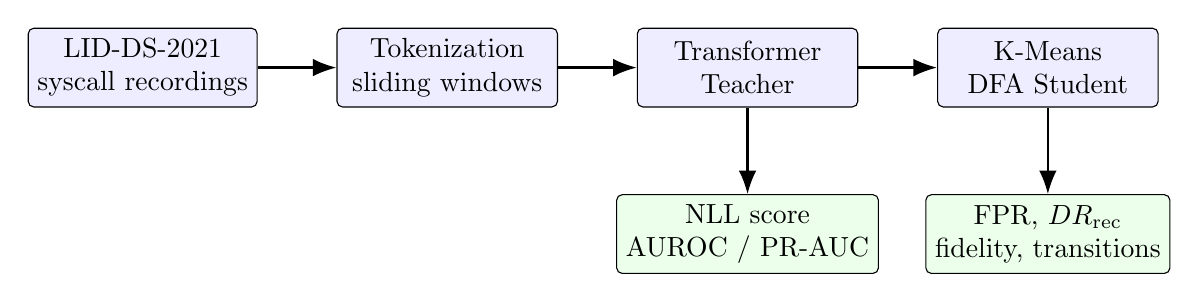
\begin{tikzpicture}[
      node distance=1.0cm,
      block/.style={rectangle, draw, rounded corners=2pt, align=center,
        minimum width=2.8cm, minimum height=1.0cm, fill=blue!7},
      result/.style={rectangle, draw, rounded corners=2pt, align=center,
        minimum width=3.0cm, minimum height=1.0cm, fill=green!8},
      arrow/.style={-{Latex[length=3mm]}, thick}
    ]
    \node[block] (raw) {LID-DS-2021\\syscall recordings};
    \node[block, right=of raw] (win) {Tokenization\\sliding windows};
    \node[block, right=of win] (teacher) {Transformer\\Teacher};
    \node[result, below=1.1cm of teacher] (p2) {NLL score\\AUROC / PR-AUC};
    \node[block, right=of teacher] (dfa) {K-Means\\DFA Student};
    \node[result, below=1.1cm of dfa] (p3) {FPR, $DR_{\mathrm{rec}}$\\fidelity, transitions};

    \draw[arrow] (raw) -- (win);
    \draw[arrow] (win) -- (teacher);
    \draw[arrow] (teacher) -- (dfa);
    \draw[arrow] (teacher) -- (p2);
    \draw[arrow] (dfa) -- (p3);
  \end{tikzpicture}
  }
  \caption{Pipeline đánh giá thực nghiệm. Transformer Teacher tạo điểm bất thường
  liên tục bằng NLL, trong khi DFA Student thay điểm số liên tục bằng kiểm tra bước
  chuyển trạng thái đã từng xuất hiện trong dữ liệu huấn luyện bình thường.}
  \label{fig:eval_pipeline}
\end{figure}

\section{Các chỉ số đánh giá}
\label{sec:eval_metrics}

Đối với Giai đoạn 2, chỉ số chính là AUROC và PR-AUC ở cấp độ window, sử dụng điểm
bất thường là negative log-likelihood (NLL) của token cuối cùng trong window. AUROC
cho biết xác suất một window attack có điểm số cao hơn một window normal khi xét trên
mọi ngưỡng có thể, còn PR-AUC phù hợp hơn trong bối cảnh tỷ lệ attack thấp hơn normal.
Ngoài ra, luận văn báo cáo ngưỡng oracle tối ưu theo F1 như một giới hạn trên lý thuyết,
nhưng không coi đây là kết quả vận hành vì ngưỡng này được chọn bằng nhãn test.

Đối với Giai đoạn 3, chỉ số trung tâm là tỷ lệ phát hiện cấp độ bản ghi
$DR_{\text{rec}}$. Chỉ số này được định nghĩa là tỷ lệ bản ghi tấn công có ít nhất
một window bị DFA từ chối:

\begin{equation}
  \label{eq:dr_rec_ch5}
  DR_{\text{rec}} =
  \frac{\text{số attack recordings có ít nhất một window bị reject}}
       {\text{tổng số attack recordings}}.
\end{equation}

Cách đo này phù hợp hơn với mục tiêu runtime của hệ thống. Khi triển khai thực tế, hệ
thống giám sát một luồng syscall liên tục và cần phát hiện thời điểm khai thác xuất
hiện, không cần gán nhãn attack cho toàn bộ phần còn lại của bản ghi. Tỷ lệ báo động
giả FPR vẫn được đo ở cấp độ window trên các window normal vì nhãn normal không chịu
cùng loại nhiễu cấu trúc như nhãn attack. Fidelity được dùng như chỉ số phụ để đo mức
đồng thuận giữa quyết định của DFA và Teacher trên tập validation.

\section{Kết quả Giai đoạn 2: Transformer Teacher}
\label{sec:p2_results}

\subsection{Cấu hình huấn luyện}
\label{subsec:p2_training_setup}

Mô hình Teacher là Transformer decoder-only với causal self-attention, được huấn luyện
theo mục tiêu dự đoán token kế tiếp trên dữ liệu bình thường. Cấu hình thực nghiệm sử
dụng $W = 64$, $d_{\text{model}} = 128$, 4 lớp Transformer, 4 attention heads,
$d_{\text{ff}} = 512$, dropout 0.1 và optimizer AdamW với learning rate $3 \times
10^{-4}$, weight decay 0.01. Lịch học sử dụng cosine decay với 5\% bước warmup, batch
size 256, mixed precision 16-bit và early stopping với patience bằng 5. Mô hình dừng ở
epoch thứ 7; validation loss tốt nhất xuất hiện tại epoch 1.

\subsection{Hội tụ huấn luyện}
\label{subsec:p2_convergence}

Bảng~\ref{tab:training_loss} và Hình~\ref{fig:training_loss_tikz} cho thấy validation
loss giảm mạnh trong epoch đầu, sau đó dao động rất nhỏ quanh mức 0.369. Train loss tiếp
tục giảm nhẹ từ 0.5292 xuống 0.3688, trong khi khoảng cách giữa train loss và validation
loss ở các epoch cuối nhỏ hơn 0.001. Diễn biến này cho thấy mô hình đã đạt trạng thái
tổng quát hóa ổn định trên tập validation bình thường và không có dấu hiệu overfitting
lớn trong cấu hình hiện tại.

\begin{table}[H]
  \caption{Diễn biến train loss và validation loss của Transformer Teacher.}
  \label{tab:training_loss}
  \centering
  \begin{tabular}{|c|c|c|}
    \hline
    \textbf{Epoch} & \textbf{Train loss} & \textbf{Validation loss} \\ \hline
    0 & 0.5292 & 0.3811 \\ \hline
    1 & 0.3830 & \textbf{0.3686} \\ \hline
    2 & 0.3762 & 0.3706 \\ \hline
    3 & 0.3732 & 0.3709 \\ \hline
    4 & 0.3713 & 0.3695 \\ \hline
    5 & 0.3699 & 0.3688 \\ \hline
    6 & 0.3688 & 0.3691 \\ \hline
  \end{tabular}
\end{table}

\begin{figure}[H]
  \centering
  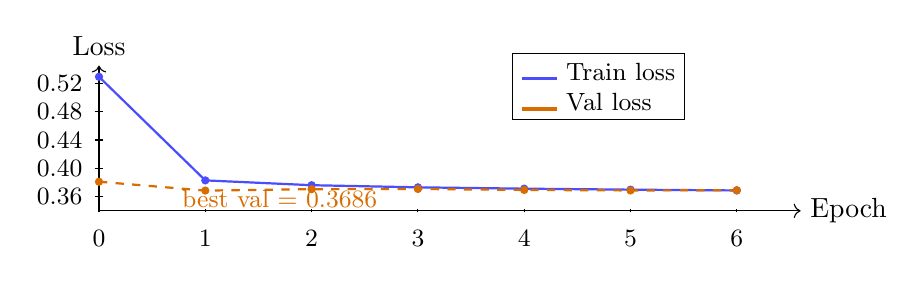
\begin{tikzpicture}[x=1.35cm, y=9cm]
    \draw[->] (0,0.34) -- (6.6,0.34) node[right] {Epoch};
    \draw[->] (0,0.34) -- (0,0.545) node[above] {Loss};
    \foreach \x in {0,1,2,3,4,5,6}
      \draw (\x,0.338) -- (\x,0.342) node[below=4pt] {\small \x};
    \foreach \y/\label in {0.36/0.36,0.40/0.40,0.44/0.44,0.48/0.48,0.52/0.52}
      \draw (-0.04,\y) -- (0.04,\y) node[left=4pt] {\small \label};

    \draw[blue!70, thick]
      plot coordinates {(0,0.5292) (1,0.3830) (2,0.3762) (3,0.3732)
        (4,0.3713) (5,0.3699) (6,0.3688)};
    \draw[orange!85!black, thick, dashed]
      plot coordinates {(0,0.3811) (1,0.3686) (2,0.3706) (3,0.3709)
        (4,0.3695) (5,0.3688) (6,0.3691)};
    \foreach \x/\y in {0/0.5292,1/0.3830,2/0.3762,3/0.3732,4/0.3713,5/0.3699,6/0.3688}
      \fill[blue!70] (\x,\y) circle (1.5pt);
    \foreach \x/\y in {0/0.3811,1/0.3686,2/0.3706,3/0.3709,4/0.3695,5/0.3688,6/0.3691}
      \fill[orange!85!black] (\x,\y) circle (1.5pt);

    \node[draw, fill=white, align=left, font=\small] at (4.7,0.515)
      {\textcolor{blue!70}{\rule{0.45cm}{1.2pt}} Train loss\\
       \textcolor{orange!85!black}{\rule{0.45cm}{1.2pt}} Val loss};
    \node[font=\small, orange!85!black] at (1.7,0.357) {best val = 0.3686};
  \end{tikzpicture}
  \caption{Đường cong hội tụ của Transformer Teacher. Validation loss đạt giá trị tốt
  nhất ở epoch 1 và sau đó đi vào vùng plateau hẹp.}
  \label{fig:training_loss_tikz}
\end{figure}

\subsection{Đánh giá cấp độ window}
\label{subsec:p2_window_eval}

Tập kiểm thử tạo ra 99,855,329 window, trong đó 82,664,861 window được gán nhãn normal
và 17,190,468 window được gán nhãn attack theo metadata của LID-DS. Điểm bất thường
chính là NLL của token cuối cùng:

\begin{equation}
  \label{eq:last_token_nll_ch5}
  \text{score}(w) = -\log P_\theta(s_W \mid s_1,\ldots,s_{W-1}).
\end{equation}

Trên tập validation bình thường, điểm số có trung bình 0.3024, phân vị 99 là 4.3359
và giá trị lớn nhất là 18.1250. Khi đánh giá trên tập test, last-token NLL đạt
AUROC = 0.8503 và PR-AUC = 0.7093. Kết quả này xác nhận rằng mô hình đã học được
phân phối hành vi bình thường đủ tốt để xếp hạng nhiều window attack cao hơn window
normal, dù không sử dụng nhãn attack trong huấn luyện.

\begin{table}[H]
  \caption{Kết quả đánh giá last-token NLL ở cấp độ window trên tập test.}
  \label{tab:p2_window_metrics}
  \centering
  \begin{tabular}{|l|c|}
    \hline
    \textbf{Chỉ số} & \textbf{Giá trị} \\ \hline
    AUROC & \textbf{0.8503} \\ \hline
    PR-AUC & \textbf{0.7093} \\ \hline
    Oracle threshold $\tau$ & 2.606 \\ \hline
    Oracle F1 (attack) & 0.80 \\ \hline
    FPR tại oracle threshold & 2.85\% \\ \hline
  \end{tabular}
\end{table}

\begin{figure}[H]
  \centering
  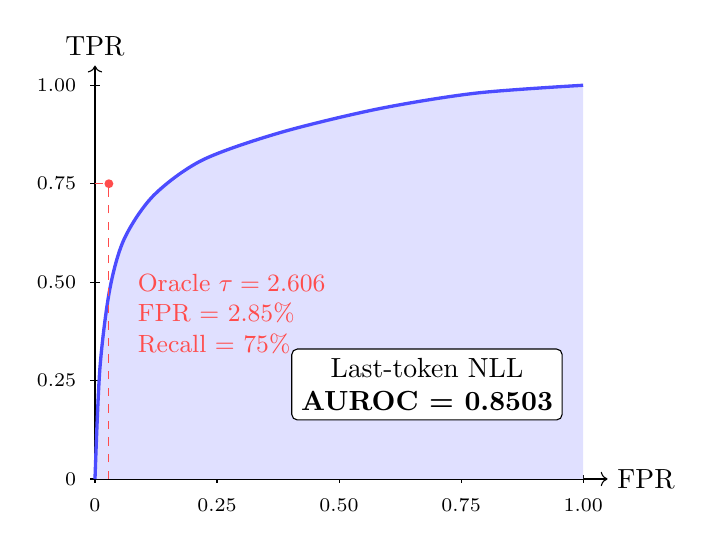
\begin{tikzpicture}[x=6.2cm, y=5.0cm]
    \draw[->] (0,0) -- (1.05,0) node[right] {FPR};
    \draw[->] (0,0) -- (0,1.05) node[above] {TPR};
    \draw[gray!60, dashed] (0,0) -- (1,1);

    \foreach \x/\label in {0/0,0.25/0.25,0.50/0.50,0.75/0.75,1.00/1.00}
      \draw (\x,-0.01) -- (\x,0.01) node[below=5pt, font=\scriptsize] {\label};
    \foreach \y/\label in {0/0,0.25/0.25,0.50/0.50,0.75/0.75,1.00/1.00}
      \draw (-0.01,\y) -- (0.01,\y) node[left=5pt, font=\scriptsize] {\label};

    \fill[blue!12]
      (0,0) -- (0.01,0.28) -- (0.03,0.48) -- (0.06,0.61) --
      (0.12,0.72) -- (0.22,0.81) -- (0.38,0.88) -- (0.58,0.94) --
      (0.78,0.98) -- (1,1) -- (1,0) -- cycle;
    \draw[blue!70, very thick]
      plot[smooth] coordinates {
        (0,0) (0.01,0.28) (0.03,0.48) (0.06,0.61)
        (0.12,0.72) (0.22,0.81) (0.38,0.88) (0.58,0.94)
        (0.78,0.98) (1,1)
      };
    \fill[red!70] (0.0285,0.75) circle (1.6pt);
    \draw[red!70, dashed] (0.0285,0) -- (0.0285,0.75);
    \draw[red!70, dashed] (0,0.75) -- (0.0285,0.75);
    \node[font=\small, red!70, align=left] at (0.28,0.42)
      {Oracle $\tau=2.606$\\FPR = 2.85\%\\Recall = 75\%};
    \node[draw, fill=white, rounded corners=2pt, align=center] at (0.68,0.24)
      {Last-token NLL\\\textbf{AUROC = 0.8503}};
  \end{tikzpicture}
  \caption{Đường cong ROC của điểm last-token NLL ở cấp độ window. Diện tích dưới đường
  cong đạt 0.8503, cho thấy Teacher xếp hạng window attack cao hơn window normal trong
  phần lớn các cặp so sánh, dù nhãn attack của LID-DS có nhiễu cấu trúc.}
  \label{fig:auroc_curve_tikz}
\end{figure}

Các biến thể ngưỡng cho thấy sự khác biệt rõ giữa năng lực xếp hạng và khả năng chọn
điểm vận hành. Nếu dùng phân vị 99.5 của validation normal, FPR chỉ khoảng 0.51\% nhưng
recall attack gần như bằng 0. Với ngưỡng oracle $\tau = 2.606$, mô hình đạt precision
attack 0.85, recall attack 0.75 và F1 attack 0.80. Vì ngưỡng oracle dùng nhãn test để
chọn điểm tối ưu, kết quả này nên được hiểu là giới hạn trên của tín hiệu Teacher thay
vì một cấu hình triển khai thực tế. Hình~\ref{fig:auroc_curve_tikz} cho thấy đường cong
ROC tổng quát của điểm NLL, còn Hình~\ref{fig:threshold_tradeoff} minh họa sự đánh đổi
precision--recall tại một số cách chọn ngưỡng cụ thể.

\begin{figure}[H]
  \centering
  \begin{tikzpicture}[x=2.2cm, y=4.2cm]
    \draw[->] (0,0) -- (3.7,0) node[right] {Ngưỡng};
    \draw[->] (0,0) -- (0,1.05) node[above] {Tỷ lệ};
    \foreach \y/\label in {0/0,0.25/0.25,0.50/0.50,0.75/0.75,1.00/1.00}
      \draw (-0.04,\y) -- (0.04,\y) node[left=4pt] {\small \label};

    \foreach \x/\p/\r/\name in {0.8/0.10/0.00/{99.5 pct},1.8/0.07/0.01/{$\mu+3\sigma$},2.8/0.85/0.75/{Oracle}}
    {
      \fill[blue!55] (\x-0.18,0) rectangle (\x-0.02,\p);
      \fill[green!55!black] (\x+0.02,0) rectangle (\x+0.18,\r);
      \node[rotate=25, anchor=east, font=\small] at (\x+0.35,-0.06) {\name};
    }
    \node[draw, fill=white, align=left, font=\small] at (2.95,0.98)
      {\textcolor{blue!55}{\rule{0.35cm}{5pt}} Precision\\
       \textcolor{green!55!black}{\rule{0.35cm}{5pt}} Recall};
  \end{tikzpicture}
  \caption{So sánh precision và recall attack tại ba cách chọn ngưỡng. Ngưỡng oracle
  thể hiện năng lực tiềm năng của điểm NLL, nhưng không phải ngưỡng vận hành vì cần
  nhãn test.}
  \label{fig:threshold_tradeoff}
\end{figure}

\subsection{Nhiễu nhãn trong LID-DS và ý nghĩa đánh giá}
\label{subsec:label_contamination}

Một kết quả quan trọng của Giai đoạn 2 là phân tích định lượng về nhiễu nhãn trong
LID-DS. Bộ dữ liệu đánh dấu toàn bộ phần tail của một bản ghi là attack kể từ
\texttt{exploit\_start}, nhưng không cung cấp thời điểm kết thúc khai thác. Vì vậy,
nhiều window nằm sau exploit thực chất chỉ chứa hành vi vận hành bình thường của server
nhưng vẫn được gán nhãn attack. Sử dụng ngưỡng oracle $\tau = 2.606$ như một proxy để
xác định các window có tín hiệu bất thường mạnh, chỉ 198,140 trong 17,190,468 labeled
attack windows vượt ngưỡng này. Điều đó tương ứng 1.15\% labeled attack windows; phần
còn lại 98.85\% là post-exploit normal behavior theo điểm số của Teacher.

\begin{figure}[H]
  \centering
  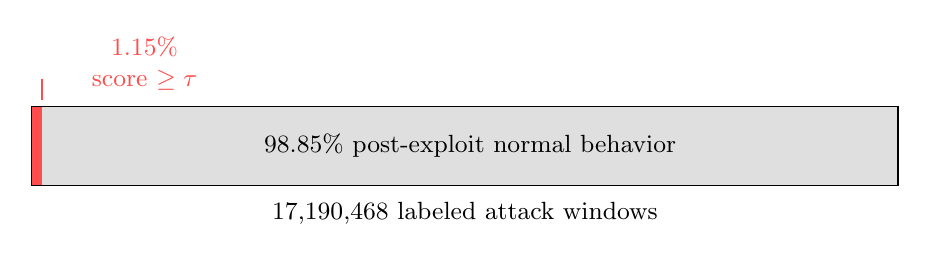
\begin{tikzpicture}[x=0.11cm, y=1cm]
    \draw[black] (0,0) rectangle (100,1);
    \fill[red!70] (0,0) rectangle (1.15,1);
    \fill[gray!25] (1.15,0) rectangle (100,1);
    \draw[black] (0,0) rectangle (100,1);
    \node[font=\small, white, rotate=90] at (0.58,0.5) {};
    \node[font=\small] at (50.6,0.5) {98.85\% post-exploit normal behavior};
    \draw[red!70, thick] (1.15,1.08) -- (1.15,1.35);
    \node[font=\small, red!70, align=center] at (13,1.55) {1.15\%\\score $\ge \tau$};
    \node[font=\small] at (50,-0.35) {17,190,468 labeled attack windows};
  \end{tikzpicture}
  \caption{Cấu trúc nhiễu nhãn trong các window được LID-DS gán nhãn attack. Phần tín
  hiệu exploit có NLL cao chỉ chiếm một tỷ lệ rất nhỏ; phần lớn tail sau khai thác có
  hành vi giống normal.}
  \label{fig:label_contamination}
\end{figure}

Kết quả này không cho phép tính một ``AUROC hiệu chỉnh'' bằng chính điểm số của mô hình,
vì thao tác đó sẽ dùng dự đoán để định nghĩa lại nhãn và dẫn tới vòng lặp suy luận. Do
đó, AUROC = 0.8503 trên nhãn thô vẫn là con số hợp lệ cần báo cáo. Tuy nhiên, cách diễn
giải phải thận trọng: nhiều mẫu positive trong phép tính AUROC thực chất không chứa tín
hiệu exploit. Ở cấp độ bản ghi, phân tích cho thấy 1,715 trong 1,815 attack recordings
được phát hiện bởi ít nhất một window vượt ngưỡng oracle, tương ứng 94.5\%. Median
detection lag trong các bản ghi phát hiện được là 14 window sau mốc \texttt{exploit\_start}.
Điều này củng cố luận điểm rằng tín hiệu tấn công trong LID-DS thường xuất hiện như một
burst ngắn, không phải một trạng thái bất thường kéo dài suốt phần tail của recording.

\subsection{Đánh giá cấp độ bản ghi}
\label{subsec:p2_recording_eval}

Để so sánh với cách đánh giá truyền thống trên LID-DS, luận văn cũng báo cáo kết quả
max-pooling điểm số theo bản ghi. Với last-token NLL, điểm của một recording là điểm
NLL lớn nhất trên tất cả các window thuộc recording đó. Ngưỡng vận hành được hiệu chuẩn
từ phân vị 99.5 của validation max-pooled score, đạt $\tau_{\text{rec}} = 15.0989$.
Ở cấp độ này, last-token NLL đạt AUROC 0.6559 và PR-AUC 0.3747; tại ngưỡng oracle
$\tau = 13.789$, F1 attack đạt 0.39 với FPR 4.70\%.

Một quan sát đáng chú ý là max-window NLL có AUROC thấp ở cấp độ window nhưng lại tốt
hơn khi max-pooled theo bản ghi, đạt AUROC 0.6997, PR-AUC 0.5490 và F1 attack 0.55 tại
ngưỡng oracle $\tau = 19.156$. Hiện tượng này phản ánh khác biệt giữa hai mục tiêu:
ở cấp độ window, một syscall hiếm trong hành vi normal có thể tạo NLL cao và gây nhiễu;
ở cấp độ recording, chỉ cần một outlier exploit đủ mạnh là điểm max-pooled của toàn bộ
bản ghi tăng lên. Tuy vậy, mục tiêu triển khai của Guepard Shield là phát hiện trên
dòng syscall liên tục tại runtime, nên recording-level aggregation chỉ được xem là
chẩn đoán bổ sung.

\section{Kết quả Giai đoạn 3: Chưng cất DFA Student}
\label{sec:p3_results}

\subsection{Thiết lập trích xuất DFA}
\label{subsec:p3_setup}

Giai đoạn 3 sử dụng các trạng thái ẩn của Transformer Teacher để tạo biểu diễn rời rạc
bằng MiniBatchKMeans. Phiên thí nghiệm hoàn chỉnh hiện tại đánh giá $K = 64$ với trạng
thái khởi đầu là cluster 59, tức cluster phổ biến nhất tại vị trí khởi đầu trong tập
train. Bảng chữ cái đầu vào khi build DFA có 816 token ID quan sát được trong pipeline
đánh giá chuyển trạng thái. NFA được dựng bằng cách stream toàn bộ tập train ở stride
1 và ghi nhận các bước chuyển dạng $(q, s) \rightarrow q'$ giữa hai vị trí syscall liên
tiếp. Khi đánh giá, mỗi window test được chạy ở chế độ cold-start, nghĩa là bắt đầu lại
từ start state. Chế độ này khắt khe hơn triển khai eBPF thực tế vì runtime sẽ duy trì
state liên tục theo từng thread thay vì reset ở mỗi window.

NFA tại $K=64$ có 1,973 cặp $(src, token)$, trong đó 85.9\% cặp có nhiều hơn một trạng
thái đích. Trung bình mỗi cặp có 7.20 đích và cặp phức tạp nhất có 30 đích. Chỉ 35 trên
64 source states hoạt động trong dữ liệu train. Tỷ lệ không đơn định cao cho thấy cụm
$K=64$ vẫn còn khá thô: một cluster có thể chứa nhiều ngữ cảnh syscall khác nhau, nên
cùng một token đầu vào từ cùng cluster có thể dẫn sang nhiều cluster tiếp theo.

\begin{figure}[H]
  \centering
  \begin{tikzpicture}[
      x=1cm, y=1cm,
      pointA/.style={circle, fill=blue!60, inner sep=1.15pt},
      pointB/.style={circle, fill=green!55!black, inner sep=1.15pt},
      pointC/.style={circle, fill=orange!85!black, inner sep=1.15pt},
      centroid/.style={star, star points=5, draw=black, fill=red!70,
        minimum size=6pt, inner sep=0pt},
      state/.style={circle, draw, fill=gray!8, minimum size=0.75cm,
        font=\small},
      arrow/.style={-{Latex[length=2.5mm]}, thick},
      panel/.style={draw, rounded corners=2pt, fill=gray!3}
    ]
    \node[panel, minimum width=5.1cm, minimum height=3.55cm] (clusterpanel)
      at (2.35,1.75) {};
    \node[font=\small] at (2.35,3.35) {K-Means trên hidden states};
    \node[font=\scriptsize] at (2.35,0.12) {$h_t \in \mathbb{R}^{128}$, minh họa sau chiếu 2D};

    \foreach \x/\y in {0.8/1.35,1.0/1.55,1.2/1.25,1.4/1.62,1.45/1.35,1.15/1.82}
      \node[pointA] at (\x,\y) {};
    \foreach \x/\y in {2.2/2.15,2.45/2.35,2.7/2.05,2.9/2.32,3.05/2.08,2.55/1.82}
      \node[pointB] at (\x,\y) {};
    \foreach \x/\y in {3.45/1.05,3.68/1.22,3.9/0.92,4.12/1.25,4.25/1.02,3.82/1.48}
      \node[pointC] at (\x,\y) {};

    \node[centroid] (c1) at (1.18,1.48) {};
    \node[centroid] (c2) at (2.65,2.15) {};
    \node[centroid] (c3) at (3.85,1.15) {};
    \node[font=\scriptsize, red!70] at (1.18,1.05) {$c_i$};
    \node[font=\scriptsize, red!70] at (2.65,2.65) {$c_j$};
    \node[font=\scriptsize, red!70] at (3.85,0.72) {$c_k$};

    \draw[arrow] (5.05,1.75) -- (6.2,1.75)
      node[midway, above, font=\small] {nearest centroid};

    \node[panel, minimum width=3.3cm, minimum height=3.55cm] (dfapanel)
      at (8.0,1.75) {};
    \node[font=\small] at (8.0,3.35) {DFA states};
    \node[state] (q1) at (7.25,2.35) {$q_i$};
    \node[state] (q2) at (8.65,2.35) {$q_j$};
    \node[state] (q3) at (8.0,1.10) {$q_k$};
    \draw[arrow] (q1) -- node[above, font=\scriptsize] {$s_a$} (q2);
    \draw[arrow] (q2) -- node[right, font=\scriptsize] {$s_b$} (q3);
    \draw[arrow] (q1) -- node[left, font=\scriptsize] {$s_c$} (q3);

    \node[draw, rounded corners=2pt, fill=green!8, align=center, font=\small,
      minimum width=2.45cm] at (8.0,0.25) {$K=64$ clusters\\$\rightarrow$ 64 states};
  \end{tikzpicture}
  \caption{Minh họa bước K-Means trong Giai đoạn 3. Các vector hidden state của Teacher
  được gom quanh các centroid, sau đó mỗi centroid được xem như một trạng thái rời rạc
  của DFA. Bảng chuyển $\delta(q,s)$ được xây dựng bằng cách quan sát các cặp trạng thái
  liên tiếp trong chuỗi syscall bình thường.}
  \label{fig:kmeans_dfa_tikz}
\end{figure}

\subsection{So sánh chiến lược giải quyết tính không xác định}
\label{subsec:p3_strategy_results}

Bốn chiến lược đã được thiết kế ở Chương 3, nhưng kết quả thực nghiệm cho thấy chỉ S3
(majority voting) là khả dụng trong cấu hình $K=64$. S1, tức subset construction từ
NFA sang DFA, gặp bùng nổ trạng thái và vượt ngưỡng cắt 10 lần $K$ trước khi tạo được
DFA gọn. S4, tức statistical pruning theo ngưỡng $\theta$, loại bỏ quá nhiều transition
do không có nhánh nào đủ thống trị trong phần lớn các cặp không đơn định. Bảng
~\ref{tab:p3_strategy_results} trình bày kết quả chi tiết.

\begin{table}[H]
  \caption{So sánh các chiến lược chưng cất DFA tại $K=64$.}
  \label{tab:p3_strategy_results}
  \centering
  \resizebox{\textwidth}{!}{
    \begin{tabular}{|l|c|c|c|c|c|}
      \hline
      \textbf{Cấu hình} & \textbf{FPR} & \textbf{$DR_{\text{rec}}$} &
      \textbf{TPR window} & \textbf{Fidelity} & \textbf{Transitions} \\ \hline
      S3 Majority Voting & \textbf{1.41\%} & 90.85\% & 0.47\% & \textbf{98.12\%} & 1,973 \\ \hline
      S4, $\theta=0.80$ & 97.57\% & 100.00\% & 25.71\% & 2.83\% & 807 \\ \hline
      S4, $\theta=0.90$ & 98.45\% & 100.00\% & 25.80\% & 1.92\% & 563 \\ \hline
      S4, $\theta=0.95$ & 98.79\% & 100.00\% & 25.85\% & 1.64\% & 440 \\ \hline
      S4, $\theta=0.99$ & 99.01\% & 100.00\% & 99.82\% & 1.45\% & 330 \\ \hline
    \end{tabular}
  }
\end{table}

\begin{figure}[H]
  \centering
  \begin{tikzpicture}[x=1.65cm, y=4.2cm]
    \draw[->] (0,0) -- (5.8,0) node[right] {Cấu hình};
    \draw[->] (0,0) -- (0,1.08) node[above] {Tỷ lệ};
    \foreach \y/\label in {0/0,0.25/25\%,0.50/50\%,0.75/75\%,1.00/100\%}
      \draw (-0.04,\y) -- (0.04,\y) node[left=4pt] {\small \label};

    \foreach \x/\fpr/\dr/\name in {
      0.7/0.014/0.909/S3,
      1.7/0.976/1.000/S4 .80,
      2.7/0.985/1.000/S4 .90,
      3.7/0.988/1.000/S4 .95,
      4.7/0.990/1.000/S4 .99}
    {
      \fill[red!60] (\x-0.18,0) rectangle (\x-0.02,\fpr);
      \fill[green!55!black] (\x+0.02,0) rectangle (\x+0.18,\dr);
      \node[rotate=25, anchor=east, font=\small] at (\x+0.30,-0.05) {\name};
    }
    \node[draw, fill=white, align=left, font=\small] at (4.6,0.22)
      {\textcolor{red!60}{\rule{0.35cm}{5pt}} FPR\\
       \textcolor{green!55!black}{\rule{0.35cm}{5pt}} $DR_{\text{rec}}$};
  \end{tikzpicture}
  \caption{Đánh đổi giữa FPR và $DR_{\text{rec}}$ của các chiến lược DFA. S4 đạt
  $DR_{\text{rec}}$ tuyệt đối bằng cách từ chối gần như toàn bộ window normal, nên
  không thể dùng trong triển khai.}
  \label{fig:p3_fpr_dr}
\end{figure}

\begin{figure}[H]
  \centering
  \resizebox{0.72\textwidth}{!}{
  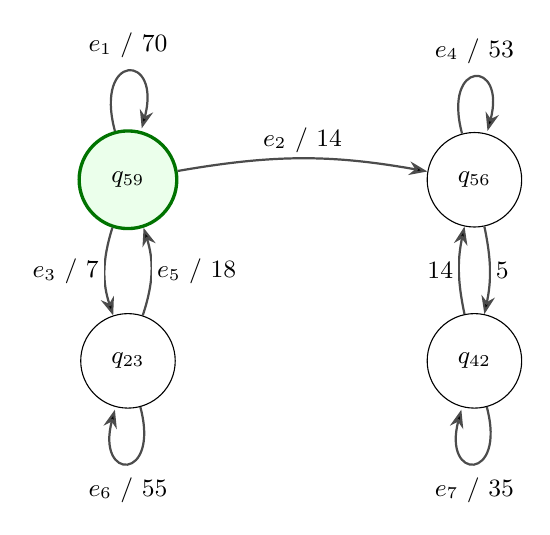
\begin{tikzpicture}[
      >=Stealth,
      state/.style={circle, draw, minimum size=1.2cm, font=\small\bfseries, fill=white},
      startstate/.style={circle, draw=green!45!black, very thick, minimum size=1.24cm,
        font=\small\bfseries, fill=green!8},
      edge/.style={->, thick, draw=black!70},
      self/.style={->, thick, draw=black!70, looseness=7},
      lab/.style={font=\small, align=center, fill=white, inner sep=1.8pt}
    ]
    \node[startstate] (q59) at (0,2.3) {$q_{59}$};
    \node[state] (q56) at (4.4,2.3) {$q_{56}$};
    \node[state] (q23) at (0,0) {$q_{23}$};
    \node[state] (q42) at (4.4,0) {$q_{42}$};

    \path[self] (q59) edge[loop above] node[lab, yshift=3pt] {$e_1$ / 70} (q59);
    \path[self] (q56) edge[loop above] node[lab, yshift=3pt] {$e_4$ / 53} (q56);
    \path[self] (q23) edge[loop below] node[lab, yshift=-3pt] {$e_6$ / 55} (q23);
    \path[self] (q42) edge[loop below] node[lab, yshift=-3pt] {$e_7$ / 35} (q42);

    \path[edge] (q59) edge[bend left=10] node[lab, above] {$e_2$ / 14} (q56);
    \path[edge] (q59) edge[bend right=18] node[lab, left] {$e_3$ / 7} (q23);
    \path[edge] (q23) edge[bend right=18] node[lab, right] {$e_5$ / 18} (q59);
    \path[edge] (q56) edge[bend left=12] node[lab, right] {5} (q42);
    \path[edge] (q42) edge[bend left=12] node[lab, left] {14} (q56);
  \end{tikzpicture}
  }
  \caption{Một graph con được lấy trực tiếp từ bảng chuyển DFA S3 tại $K=64$. Mỗi
  cạnh gom các dòng có cùng cặp state nguồn--đích; nhãn trên cạnh có dạng mã cạnh /
  số syscall token. Start state của bảng chuyển là $q_{59}$ và toàn bộ DFA S3 có
  1,973 transitions.}
  \label{fig:p3_dfa_transition_sample}
\end{figure}

\begin{table}[H]
  \caption{Chú giải các cạnh chính trong graph con DFA ở Hình~\ref{fig:p3_dfa_transition_sample}.}
  \label{tab:p3_dfa_edge_sample}
  \centering
  \resizebox{\textwidth}{!}{
    \begin{tabular}{|c|c|c|l|}
      \hline
      \textbf{Cạnh} & \textbf{State transition} & \textbf{Số token} & \textbf{Token đại diện} \\ \hline
      $e_1$ & $q_{59}\rightarrow q_{59}$ & 70 & \texttt{accept}, \texttt{close}, \ldots \\ \hline
      $e_2$ & $q_{59}\rightarrow q_{56}$ & 14 & \texttt{connect}, \texttt{madvise}, \ldots \\ \hline
      $e_3$ & $q_{59}\rightarrow q_{23}$ & 7 & \texttt{fsync}, \texttt{shutdown}, \ldots \\ \hline
      $e_4$ & $q_{56}\rightarrow q_{56}$ & 53 & \texttt{clone}, \texttt{connect}, \ldots \\ \hline
      $e_5$ & $q_{23}\rightarrow q_{59}$ & 18 & \texttt{clone}, \texttt{pipe}, \ldots \\ \hline
      $e_6$ & $q_{23}\rightarrow q_{23}$ & 55 & \texttt{fsync}, \texttt{fcntl}, \ldots \\ \hline
      $e_7$ & $q_{42}\rightarrow q_{42}$ & 35 & \texttt{epoll\_wait}, \texttt{fcntl}, \ldots \\ \hline
    \end{tabular}
  }
\end{table}

S3 đạt FPR 1.41\%, $DR_{\text{rec}}$ 90.85\% và fidelity 98.12\% với Teacher. Đây là
cấu hình cân bằng nhất trong phiên thí nghiệm hiện tại: cứ khoảng 71 window normal mới
có một window bị báo nhầm, trong khi hơn 9 trên 10 recording tấn công có ít nhất một
window bị từ chối. Hình~\ref{fig:p3_dfa_transition_sample} minh họa cách đọc bảng
chuyển S3 bằng một graph con quanh start state $q_{59}$. Chẳng hạn, các dòng
$(q_{59}, \texttt{accept}) \mapsto q_{59}$ và
$(q_{59}, \texttt{close}) \mapsto q_{59}$ nằm trong self-loop 70 token của
$q_{59}$, trong khi các syscall như \texttt{connect} hoặc \texttt{madvise} chuyển
sang $q_{56}$. Vì vậy DFA không chỉ lưu một danh sách syscall hợp lệ toàn cục, mà
lưu ngữ cảnh: cùng một syscall có thể được chấp nhận ở nhiều state khác nhau nhưng
dẫn tới hidden-state cluster khác nhau tùy lịch sử trước đó. TPR window của S3 chỉ
0.47\%, nhưng con số này không mâu thuẫn với
$DR_{\text{rec}}$ cao. Như đã phân tích ở Mục~\ref{subsec:label_contamination}, phần
lớn labeled attack windows thực chất là post-exploit normal behavior; một DFA đúng nên
chấp nhận các window đó thay vì cố gắng reject toàn bộ tail được gán nhãn attack.

S4 thất bại vì giả thuyết phân phối transition bị lệch mạnh chưa đúng ở $K=64$. Với
ND rate 85.9\%, phần lớn cặp $(q, s)$ có nhiều đích nhưng không có đích nào chiếm tỷ lệ
đủ cao để vượt ngưỡng $\theta$. Khi $\theta = 0.80$, S4 chỉ giữ lại 807 trong 1,973
transition, tương đương khoảng 41\% bảng chuyển ban đầu. Các chuỗi normal vì vậy liên
tục gặp missing transition và bị reject, làm FPR tăng lên 97.57\%. Khi tăng $\theta$,
bảng chuyển càng nhỏ và fidelity càng giảm. Kết quả này đảo ngược kỳ vọng ban đầu rằng
statistical pruning sẽ là ứng viên chính; trong cấu hình hiện tại, majority voting mới
là lựa chọn thực tế.

\subsection{Kích thước DFA và tính khả thi eBPF}
\label{subsec:p3_ebpf_feasibility}

Cấu hình S3 tại $K=64$ tạo ra 64 states và 1,973 transitions. Nếu biểu diễn bảng chuyển
dưới dạng mảng trực tiếp kích thước $64 \times 816$ với mỗi ô lưu một số nguyên 32-bit,
dung lượng lý thuyết xấp xỉ:

\begin{equation}
  \label{eq:p3_bpf_memory}
  64 \times 816 \times 4 = 208{,}896 \text{ bytes} \approx 204 \text{ KB}.
\end{equation}

Mức bộ nhớ này nhỏ hơn rất nhiều so với giới hạn thực tế của BPF maps trên các hệ thống
Linux hiện đại và phù hợp với phân tích lý thuyết ở Chương 4. Nếu dùng hash map thưa,
số entry thực sự chỉ là 1,973, nên bộ nhớ còn thấp hơn nữa, đổi lại phải trả chi phí
hash lookup. Trong cả hai phương án, logic runtime vẫn giữ dạng $O(1)$: đọc trạng thái
hiện tại của thread, tra cứu token syscall, lấy trạng thái kế tiếp, và reject nếu không
tồn tại transition hợp lệ.

\begin{figure}[H]
  \centering
  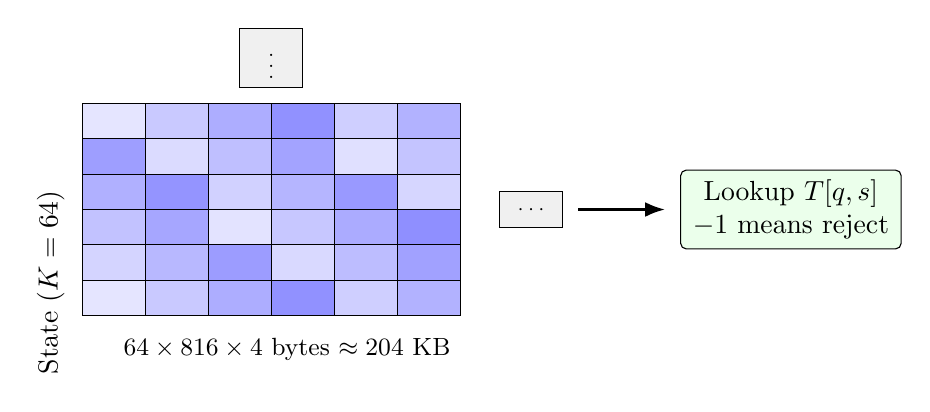
\begin{tikzpicture}[
      cell/.style={rectangle, draw, minimum width=0.8cm, minimum height=0.45cm,
        font=\scriptsize},
      arrow/.style={-{Latex[length=2.5mm]}, thick}
    ]
    \node[align=center] at (2.4,2.1) {Token ID ($|\Sigma|=816$)};
    \node[rotate=90, align=center] at (-0.8,0.2) {State ($K=64$)};
    \foreach \i in {0,...,5} {
      \foreach \j in {0,...,5} {
        \pgfmathtruncatemacro{\shade}{10+mod(\i*7+\j*11,35)}
        \node[cell, fill=blue!\shade] at (\j*0.8,\i*0.45) {};
      }
    }
    \node[cell, fill=gray!12] at (5.3,1.125) {$\cdots$};
    \node[cell, fill=gray!12] at (2.0,3.05) {$\vdots$};
    \draw[arrow] (5.9,1.125) -- (7.0,1.125);
    \node[draw, rounded corners=2pt, align=center, fill=green!8, minimum width=2.8cm,
      minimum height=1.0cm] at (8.6,1.125)
      {Lookup $T[q,s]$\\$-1$ means reject};
    \node[font=\small, align=center] at (2.2,-0.65)
      {$64 \times 816 \times 4$ bytes $\approx 204$ KB};
  \end{tikzpicture}
  \caption{Biểu diễn bảng chuyển DFA dưới dạng mảng trực tiếp. Kích thước của cấu hình
  S3 đủ nhỏ để nạp vào BPF map và cho phép tra cứu trạng thái kế tiếp bằng một phép
  chỉ mục hóa hằng số.}
  \label{fig:bpf_table}
\end{figure}

\subsection{Giới hạn của thí nghiệm Giai đoạn 3}
\label{subsec:p3_limits}

Kết quả Giai đoạn 3 hiện mới đánh giá đầy đủ cấu hình $K=64$. Các cụm $K=128$, $K=256$
và $K=512$ đã có artifact centroid và label, nhưng grid search chất lượng cao chưa hoàn
tất cho toàn bộ miền tham số. Quan sát ban đầu cho thấy MiniBatchKMeans ở $K=128$ với
cấu hình nhẹ có tỷ lệ empty clusters cao, nên cần chạy lại clustering với số lần khởi
tạo và batch size lớn hơn trước khi so sánh công bằng. Vì vậy, kết luận thực nghiệm
của chương này nên được hiểu là xác nhận tính khả thi của pipeline P3 và chỉ ra cấu
hình khả dụng đầu tiên, không phải tối ưu toàn cục của không gian $K$ và $\theta$.

Một giới hạn khác là chế độ đánh giá cold-start ở cấp độ window. Chế độ này phù hợp để
so sánh các chiến lược DFA trong điều kiện tái lập, nhưng khác với triển khai runtime,
nơi state được giữ liên tục theo từng TID. Cold-start có thể làm tăng FPR vì mỗi window
bắt đầu từ cùng một start state thay vì từ trạng thái lịch sử thực sự của luồng. Do đó,
FPR 1.41\% của S3 nên được xem là một ước lượng thận trọng cho pipeline hiện tại; đánh
giá eBPF streaming ở Giai đoạn 4 vẫn cần được thực hiện để đo độ trễ và FPR vận hành.

\section{Thảo luận tổng hợp}
\label{sec:ch5_discussion}

Các kết quả thực nghiệm xác nhận ba điểm chính của thiết kế Guepard Shield. Thứ nhất,
Transformer Teacher học được manifold hành vi bình thường từ dữ liệu không giám sát và
tạo ra điểm NLL có khả năng xếp hạng bất thường rõ rệt, thể hiện qua AUROC 0.8503 và
PR-AUC 0.7093 trên gần 100 triệu window test. Thứ hai, phân tích nhiễu nhãn cho thấy
đánh giá raw per-window trên LID-DS cần được diễn giải cẩn thận: 98.85\% window được
gán nhãn attack thực chất giống hành vi bình thường sau khai thác, nên chỉ số phát hiện
phù hợp hơn cho DFA là $DR_{\text{rec}}$. Thứ ba, pipeline chưng cất DFA có thể tạo ra
một Student rất nhỏ, chỉ 64 states và 1,973 transitions, nhưng vẫn đạt $DR_{\text{rec}}$
90.85\%, FPR 1.41\% và fidelity 98.12\% khi dùng majority voting.

Kết quả cũng điều chỉnh một giả định thiết kế ban đầu. Chương 3 kỳ vọng statistical
pruning S4 sẽ tận dụng phân phối syscall lệch mạnh để loại bỏ nhiễu lượng tử hóa. Thực
nghiệm tại $K=64$ cho thấy điều ngược lại: vì cluster còn thô, non-determinism quá rộng
và không có nhánh đủ thống trị để pruning giữ lại. Điều này không phủ nhận giá trị của
S4 ở các cấu hình $K$ lớn hơn, nhưng đặt ra yêu cầu thực nghiệm rõ ràng cho bước tiếp
theo: cần hoàn thành grid search trên $K \in \{128, 256, 512\}$ với clustering chất
lượng cao hơn để kiểm tra liệu tỷ lệ không đơn định có giảm đủ để S4 trở nên khả dụng.

Từ góc nhìn triển khai, cấu hình S3 hiện tại đã đáp ứng mục tiêu quan trọng nhất của
luận văn: chuyển một mô hình Teacher nặng, hoạt động trên không gian vector liên tục,
thành một bảng chuyển trạng thái nhỏ có thể kiểm tra bằng số nguyên trong kernel. Phần
chưa hoàn tất là đánh giá Giai đoạn 4 trên eBPF thật, bao gồm overhead trên mỗi syscall,
FPR trong workload bình thường liên tục và hành vi cập nhật khi gặp trạng thái Edge.
Do đó, chương này nên được xem là bằng chứng thực nghiệm cho tính khả thi của chưng
cất Transformer-to-DFA, đồng thời đặt nền tảng định lượng cho phần kết luận và hướng
phát triển tiếp theo.

\end{document}
